\documentclass[11pt]{article}
\usepackage[utf8]{inputenc}
\usepackage{amsmath, amssymb}
\usepackage{graphicx}
\usepackage{hyperref}
\usepackage{geometry}
\geometry{margin=1in}

\title{Expanding Entropy and the Birth of Spacetime}
\author{Juha}
\date{\today}

\begin{document}
\maketitle


\begin{abstract}
   We explore the hypothesis that the growth of entropy in a computable execution trace corresponds to the expansion of spacetime,
   offering a natural explanation for the low-entropy initial state of the universe and its inflationary growth. Using simple simulations
   based on bit string evolution and particle definitions from minimal structures, we demonstrate that entropy
   increase drives an emergent geometric expansion. Furthermore, we uncover that the statistical distribution of emergent
   structure probability follows a lognormal pattern.
\end{abstract}

\section{Introduction}

Why did the universe begin in such a finely tuned state? And why does entropy continue to increase as the universe expands?
These questions have often been treated as separate, but we argue that they are fundamentally linked.
In our previous work, we proposed an information-theoretic framework to describe the collapse of spacetime geometry through
the lens of entropy reduction, formalized in the **Entropy-Singularity Lemma**: *vanishing entropy implies geometric
singularity* \cite{Paper1}.

In this paper, we reverse this process, postulating that the **increase in entropy** corresponds to the expansion of spacetime,
effectively mapping the increase in informational complexity to cosmological expansion.


\section{Entropy as a Driver of Expansion}

We define an execution trace ${S_t}_{t=0}^n$, where each $S_t$ is a binary string of fixed length $L$.
Starting from a state of zero entropy (all-zero string), we evolve $S_t$ forward using a random bit-flip mutation process that
incrementally increases entropy.

Each $S_t$ is interpreted geometrically through a decoding scheme $D: \{0,1\}^L \to \mathbb{R}^d$. In this study,
we define the hierarchy of elementary structures as follows:

1. **Spacetime fabric**, as directly defined by 3D points encoded from the bistring.

2. **Elementary Particles:** These are defined as pairs of 3D points, i.e., pairs of
coordinates $((x_1, y_1, z_1), (x_2, y_2, z_2))$, where the spatial separation between the
points is fixed. Specifically, an elementary particle is formed when two points in the 3D space are within
a certain threshold distance, indicating that they can be considered a pair of interacting points.

3. **Atoms:** We define an atom as a set of three points $(p_1, p_2, p_3)$ where the distances between the points satisfy:
\[
   0 < \text{distance}(p_1, p_2) < \text{threshold}, \quad 0 < \text{distance}(p_2, p_3) < \text{threshold}, \quad 0 < \text{distance}(p_3, p_1) < \text{threshold},
\]
and the distances are sufficiently close to each other such that the structure is nearly equilateral

4. **Molecules:** A molecule is formed when two atoms are sufficiently close in space, with the distance between
their centers being below a given threshold. The center of an atom is defined as the geometric center of the three points forming the atom:
\[
   \text{center}(atom) = \left( \frac{x_1 + x_2 + x_3}{3}, \frac{y_1 + y_2 + y_3}{3}, \frac{z_1 + z_2 + z_3}{3}, \frac{t_1 + t_2 + t_3}{3} \right).
\]
A molecule is considered to be formed when the distance between the centers of two atoms, $atom_1$ and $atom_2$, is below a threshold value:
\[
   \text{distance}(\text{center}(atom_1), \text{center}(atom_2)) < \text{threshold}.
\]
Thus, a molecule is a structure consisting of two atoms in close proximity, representing the next level of complexity in the hierarchy.


We define a decoding rule that extracts these particles from substrings of $S_t$, and count the number of distinct particles
present at each timestep. We simulate the evolution of $S_t$ by applying random bit flips, which increase the Shannon entropy of the string.
We find:

\begin{enumerate}
   \item Initially, when entropy is near zero, no valid particles are decoded.
   \item As entropy increases, particle count grows exponentially.
   \item This exponential rise slows as entropy increases further, matching the inflationary burst followed by slower expansion.
\end{enumerate}


\begin{figure}[h!]
   \centering
   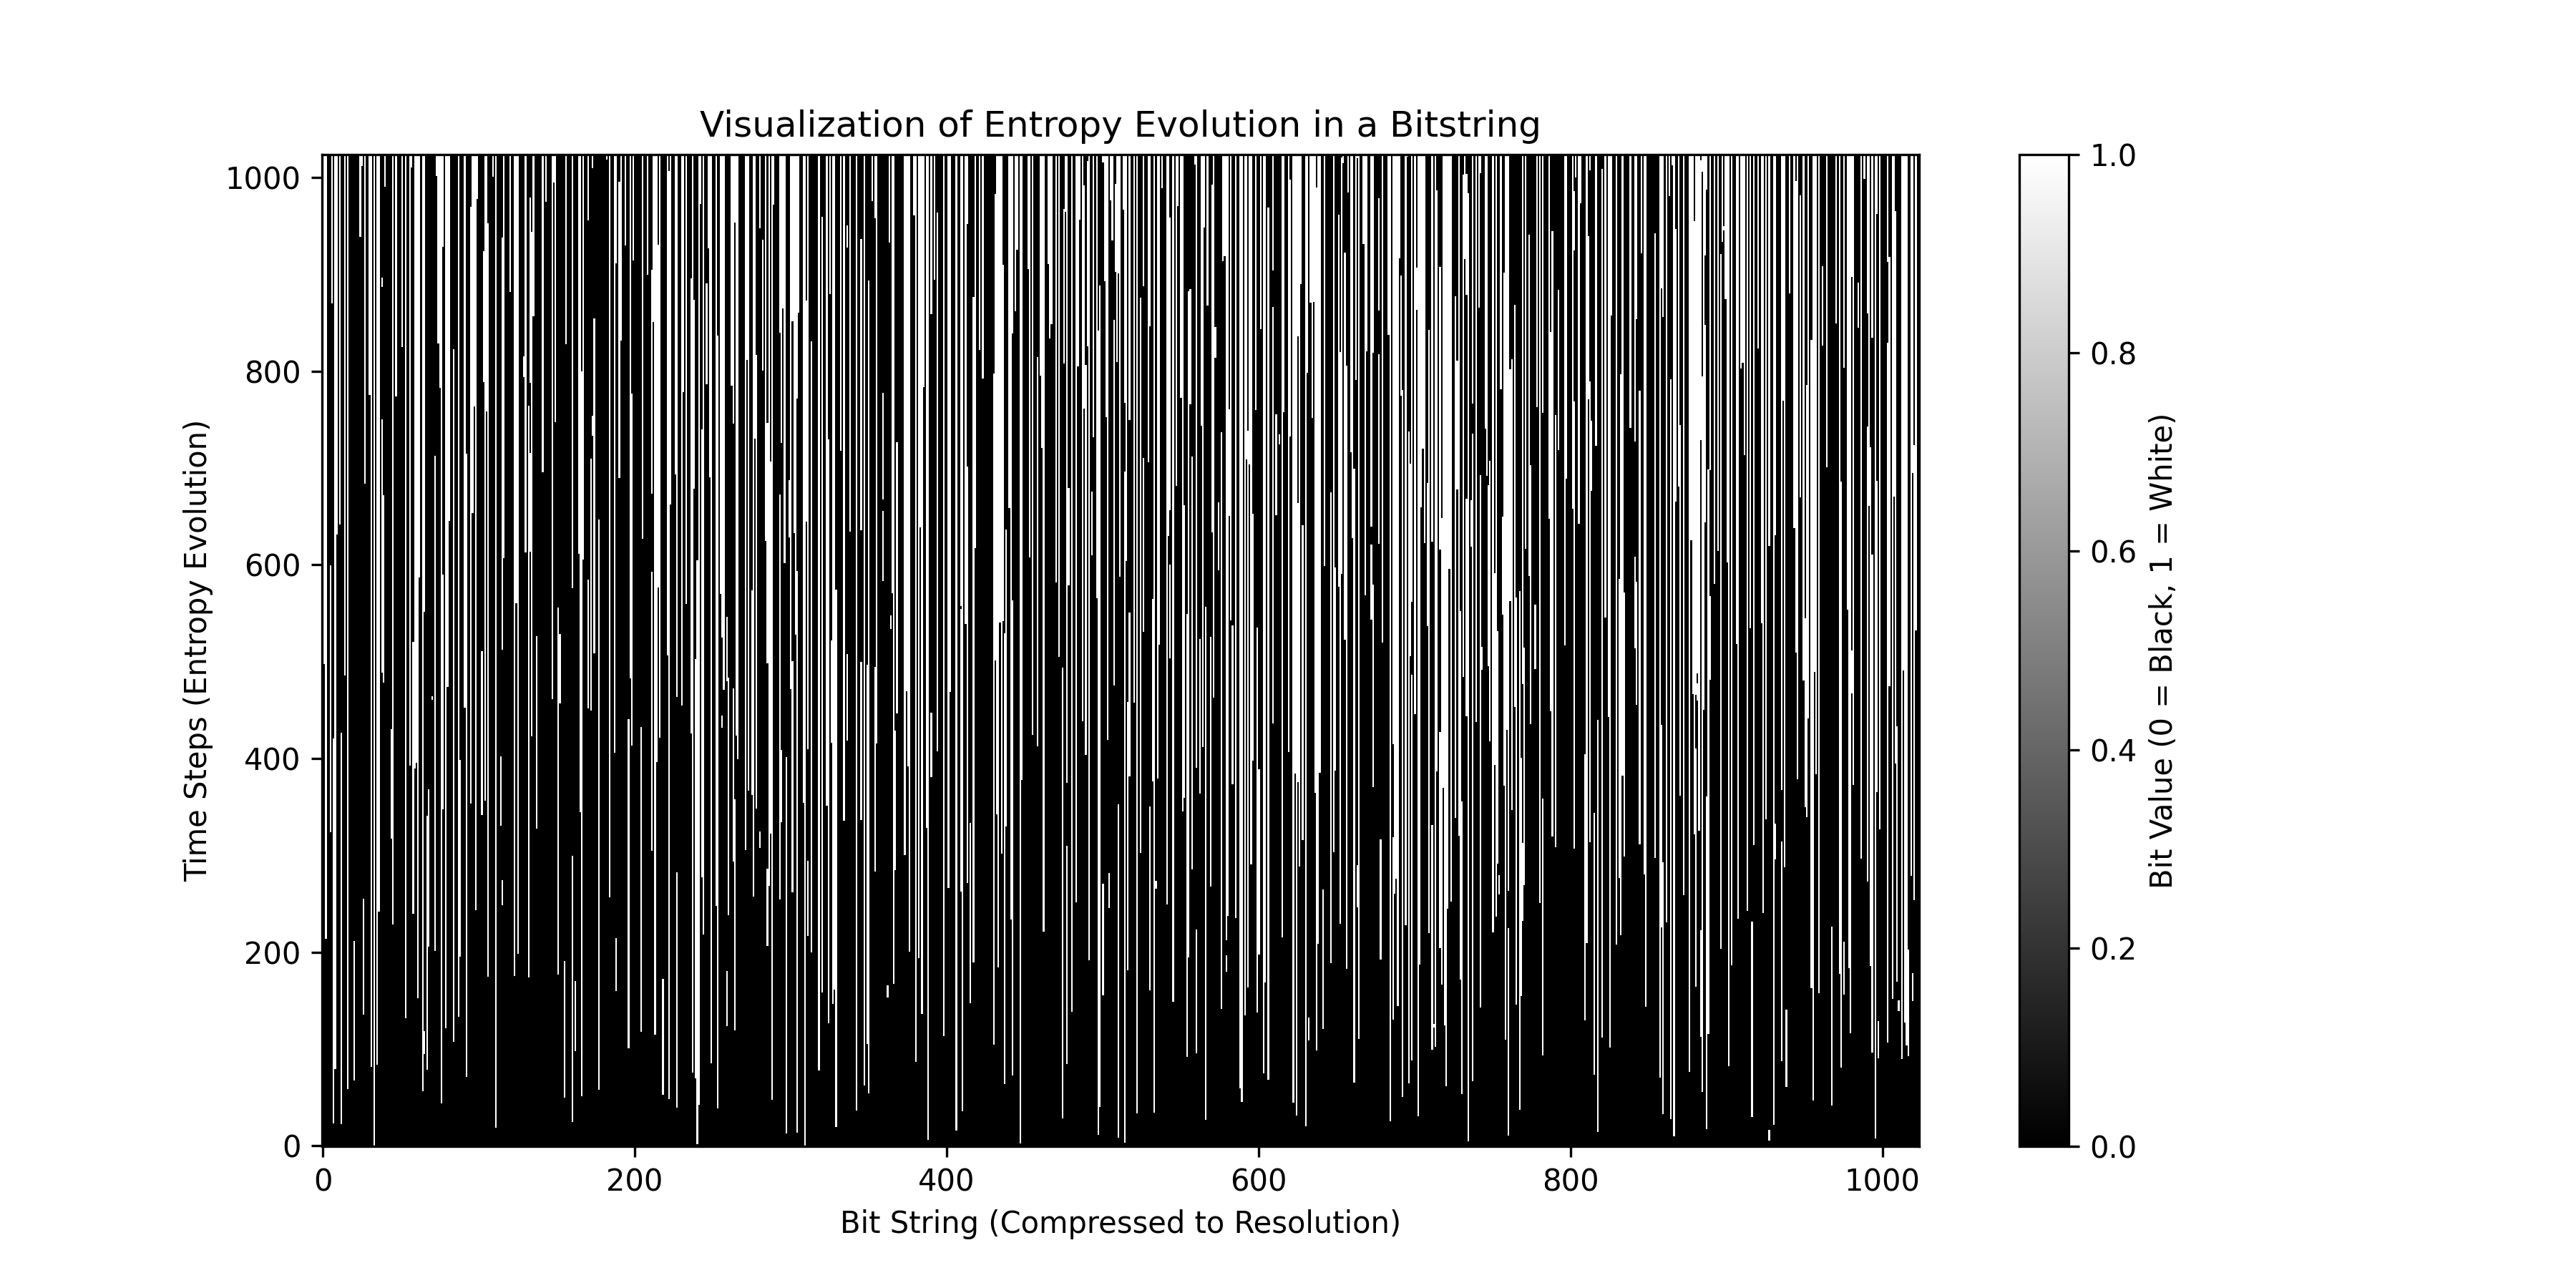
\includegraphics[width=0.8\textwidth]{entropy_evolution_image.png}
   \caption{Evolution of Shannon entropy due to bit-flips.}
   \label{fig:Evolution of entropy due to bit-flips}
\end{figure}


\begin{figure}[h!]
   \centering
   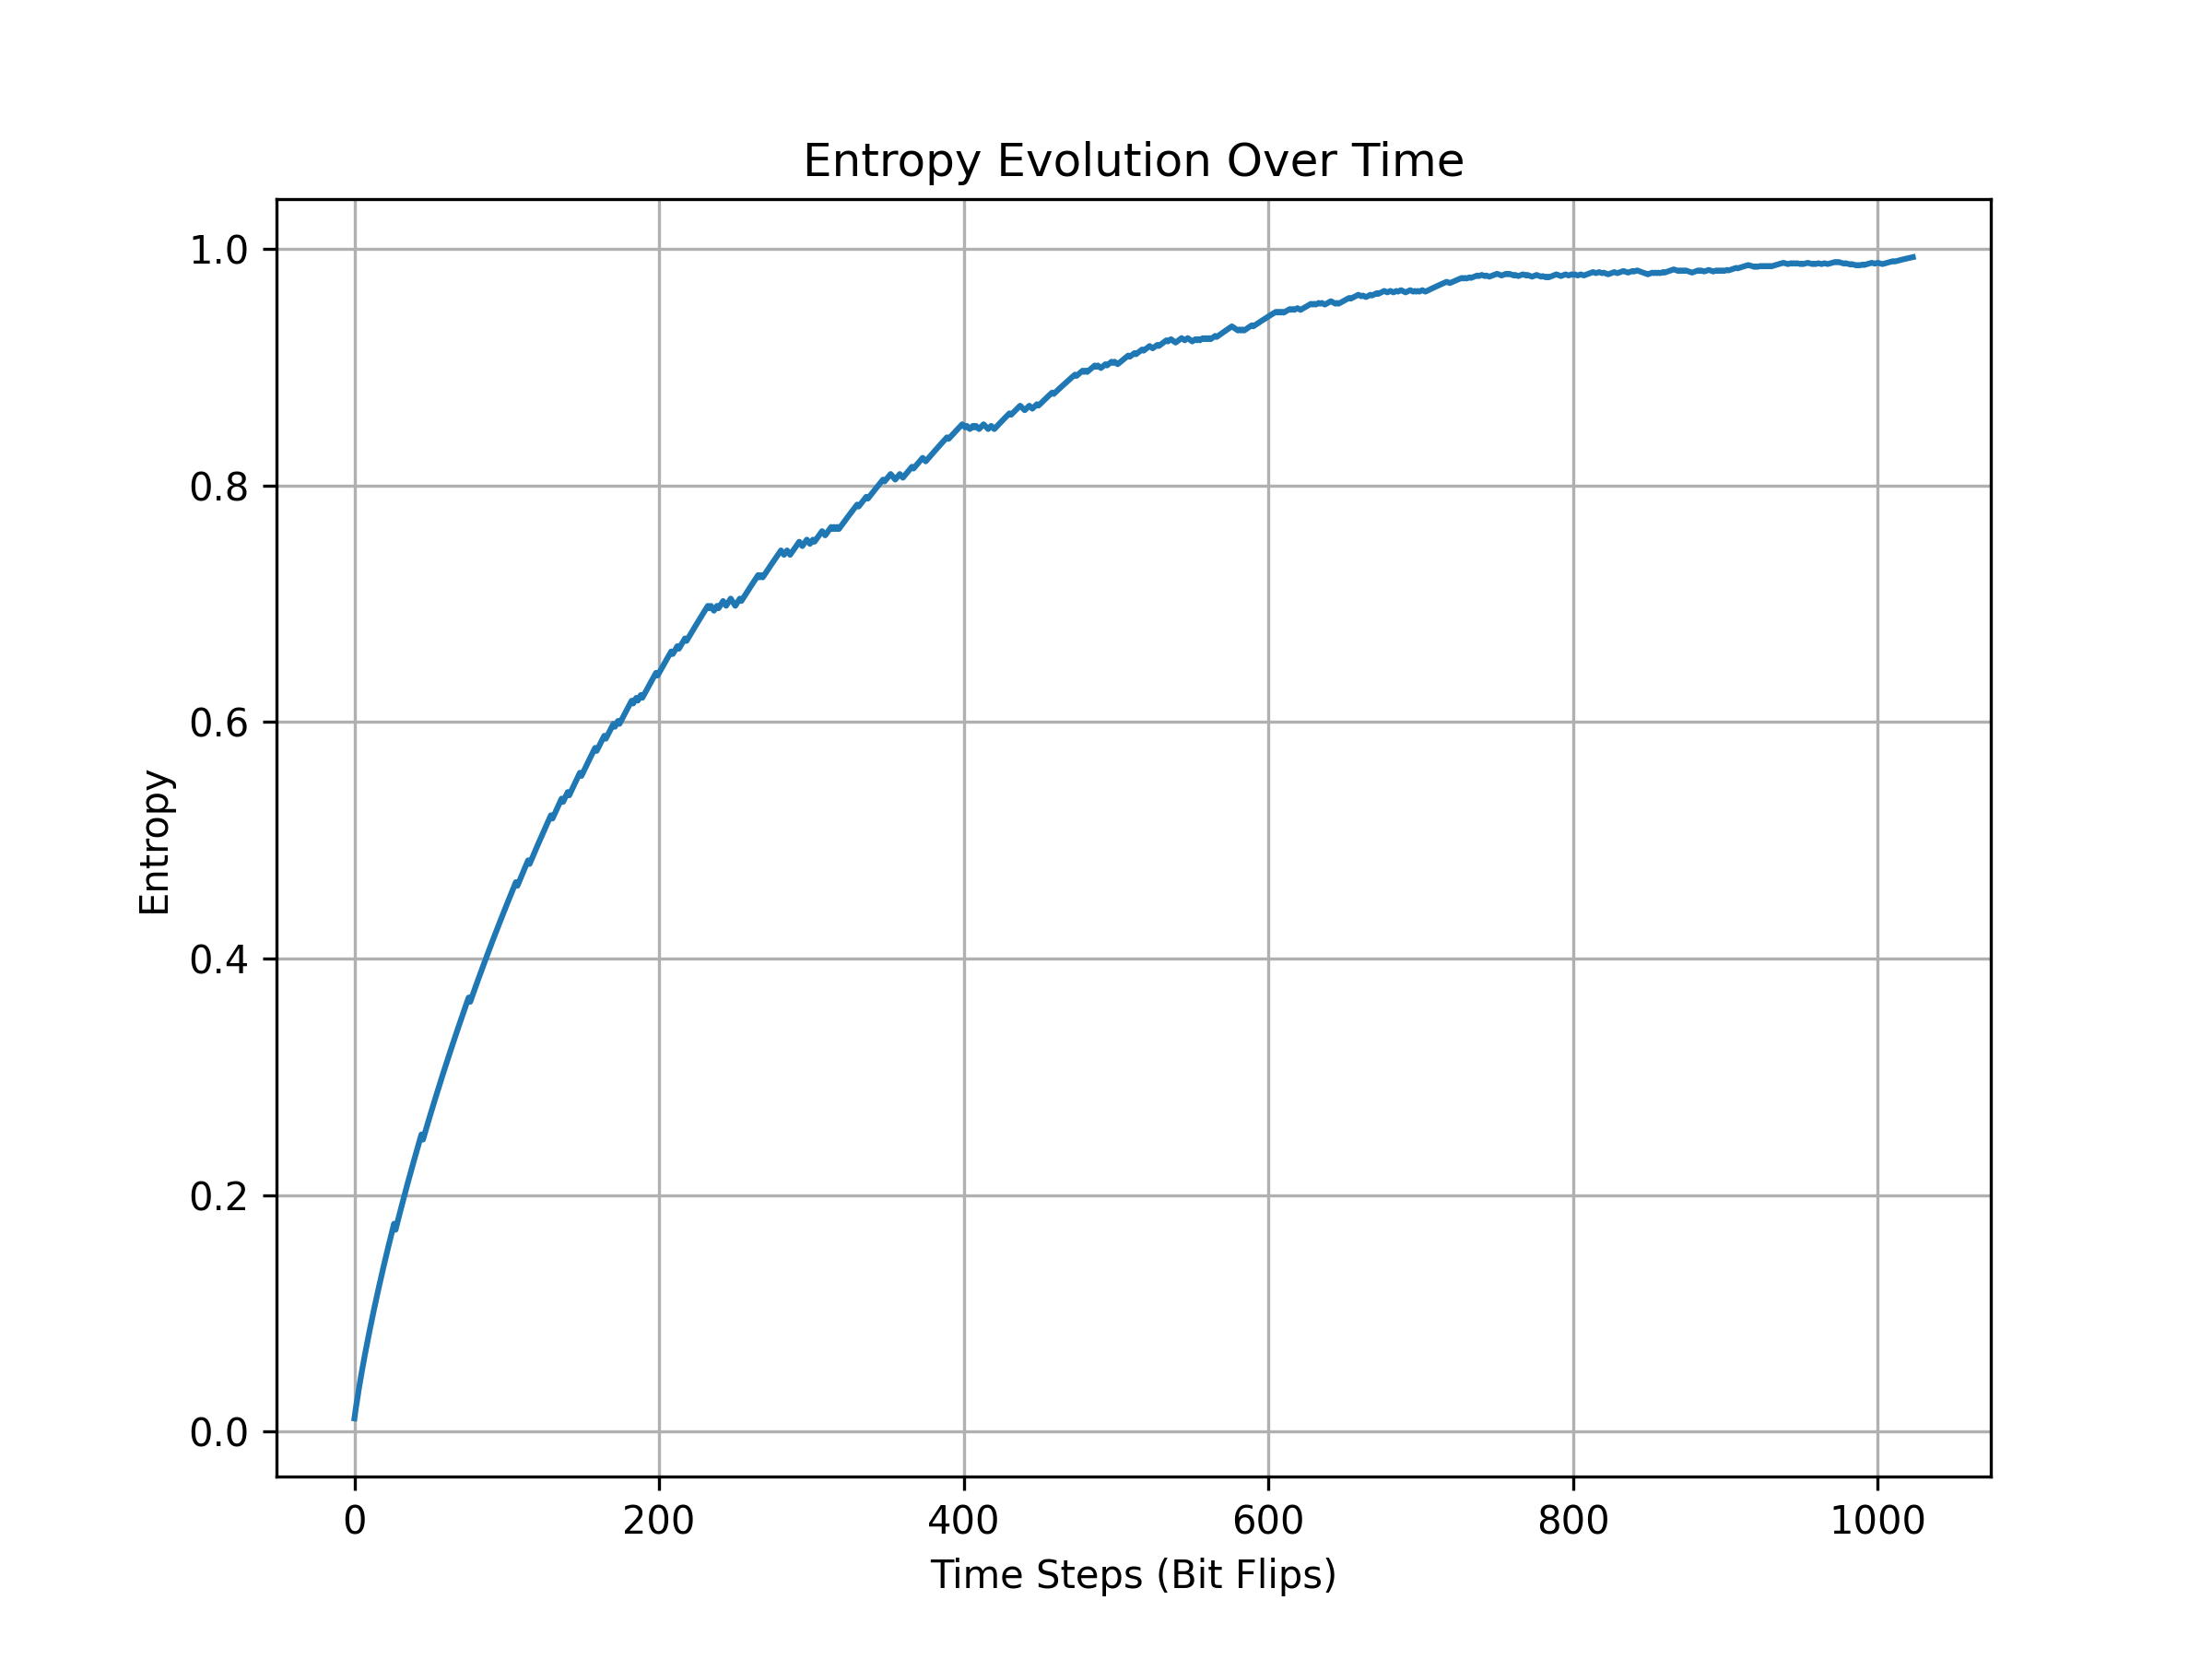
\includegraphics[width=0.8\textwidth]{entropy_evolution_curve.png}
   \caption{Evolution of bitstrings}
   \label{fig:Evolution of bitstrings due to bit-flips}
\end{figure}

\section{Statistical Properties: Lognormal Emergence}
Plotting the number of valid geometric interpretations (particles) against entropy yields a distribution resembling a lognormal curve:
\begin{itemize}
   \item Rapid rise in structure during early entropy increase.
   \item Peak structure formation at intermediate entropy.
   \item Long-tailed saturation as entropy nears maximum.
\end{itemize}

This aligns with observed cosmic evolution: inflation (early burst), structure formation, and degeneration during late-time
when the entropy reaches its maximum.

The results also show that at lower entropy, only elementary particles exist, while at higher entropy, atoms and molecules emerge.
The curves depicting these structures provide insight into the relationship between entropy and complexity, highlighting
the natural progression from simple to complex forms as entropy increases.

\begin{figure}[h!]
   \centering
   \includegraphics[width=0.8\textwidth]{emergence_plot_with_unique_points.png}
   \caption{Simulated structure count as a function of entropy in the execution trace. The emergence follows a lognormal-like distribution.}
   \label{fig:lognormal-structure}
\end{figure}

The simulation program is hosted at \url{http://github.com/juhakm/emergence_of_spacetime.py}.

\section\*{Discussion}

This model, despite its simplicity and lack of predictive power, reveals surprising regularities in the evolution of bitstring-based
universes. One of the most striking is the emergence of a lognormal distribution in the frequency of structures near the entropy minimum. This distribution has a direct geometric interpretation: it implies that the singularity is not a point of physical breakdown, but of perfect informational smoothness. In such a regime, the entropy landscape offers no persistent structures—hence, no particles, no time evolution, no memory.

This stands in sharp contrast to both General Relativity, which predicts infinite curvature at the singularity, and Quantum Mechanics, which denies the very possibility of a well-defined state with zero entropy. Yet our simulation begins precisely with such a state and shows that coherent structure emerges only as entropy increases.

We suggest this contradiction is not a failure of the simulation, but a sign that the prevailing physical theories are incomplete—or perhaps even misdirected at fundamental scales.

\section\*{Conclusion}

Our findings suggest that both GR and QM break down at the singularity not because the mathematics becomes difficult, but because the assumptions of those theories are inapplicable to a universe that is fundamentally informational. Rather than infinities or quantum fluctuations, we find a well-defined, smooth entropy profile—one that gives rise to spacetime and matter only after entropy begins to rise. In this view, spacetime is not the arena in which information evolves; rather, information is the substance from which spacetime emerges.
Spacetime is a geometric interpretation of the entropy landscape, and particles are emergent structures that arise from the information encoded in bitstrings.




\section{Future Work}

This paper establishes a computational framework in which entropy increase corresponds to the emergence of spacetime geometry and structure, offering a clean statistical alternative to the singular initial conditions postulated by General Relativity and Quantum Mechanics.

Future work will extend this model in several directions:

\begin{itemize}
   \item \textbf{Unified Replacement for GR and QM:} We will explore the implications of the observed breakdown of both GR (due to singularities) and QM (due to the assumption of nonzero entropy at origin), and construct a unified information-theoretic framework to describe phenomena attributed to spacetime curvature and quantum entanglement.

   \item \textbf{Emergence of Consciousness:} No theory can be regarded as Theory of Everything, unless it includes also human conduct. We explore how subjective experience and stable physics emerge only in a narrow class of such simulations, accounting for the apparent fine-tuning of our universe without invoking external causes.

   \item \textbf{Empirical Consequences and Falsifiability:} Although the current simulation is abstract, we will discuss how this model could be falsified or confirmed indirectly, for instance through the entropy distribution of observed microstructure or the breakdown of existing physical laws near black hole singularities.
\end{itemize}

Ultimately, we aim to replace geometric and probabilistic descriptions of the universe with a single, consistent, observer-relative model grounded in finite information and computability.


\end{document}

